% UICTEST.TEX
% This is a test file for my port of UICTHESI
% to LaTeX 2e. This is based in part on UCTHESIS.
%

\documentclass{uicthesi}




\usepackage{booktabs} % For formal tables

\usepackage{framed}
\usepackage{hyperref}
\usepackage{balance}
\usepackage[dvips]{graphics,color}
\usepackage{tabularx}

\usepackage{epsfig}
\usepackage{color}
\usepackage{subfigure}
\usepackage{multirow,tabularx}
\usepackage{placeins}
%\usepackage{miniltx}
\usepackage{mathtools}
\usepackage{graphicx}
\usepackage{epstopdf}
\usepackage{bm}

\usepackage{csquotes}
\usepackage{array}
\usepackage[yyyymmdd,hhmmss]{datetime}
\usepackage[subject={Todo}]{pdfcomment}
\usepackage[textsize=scriptsize,bordercolor=black!20]{todonotes}
\usepackage{xcolor,colortbl}
\usepackage{amssymb}% http://ctan.org/pkg/amssymb
\usepackage{pifont}% http://ctan.org/pkg/pifont
\usepackage[algo2e,titlenumbered,ruled]{algorithm2e} 
\usepackage{lipsum,environ,amsmath}
\usepackage{slashbox,booktabs,amsmath}
%\usepackage{todonotes}
\usepackage{cite}

\usepackage{xspace}

\hyphenation{PageRank Convex dictatorship Dic-ta-tor-ship}

\newcounter{Lcount}
\newcommand{\numsquishlist}{
   \begin{list}{\arabic{Lcount}. }
    { \usecounter{Lcount}
 \setlength{\itemsep}{-.1ex}      \setlength{\parsep}{0ex}
      \setlength{\topsep}{0ex}       \setlength{\partopsep}{0ex}
      \setlength{\leftmargin}{1em} \setlength{\labelwidth}{1em}
      \setlength{\labelsep}{0.1em} } }
\newcommand{\numsquishend}{\end{list}}

\newcommand{\squishlist}{
   \begin{list}{$\bullet$}
    { \setlength{\itemsep}{-.1ex}      \setlength{\parsep}{0ex}
      \setlength{\topsep}{0ex}       \setlength{\partopsep}{0ex}
      \setlength{\leftmargin}{.8em} \setlength{\labelwidth}{1em}
      \setlength{\labelsep}{0.5em} } }
\newcommand{\squishend}{\end{list}}



\makeatletter
\DeclareOldFontCommand{\rm}{\normalfont\rmfamily}{\mathrm}
\DeclareOldFontCommand{\sf}{\normalfont\sffamily}{\mathsf}
\DeclareOldFontCommand{\tt}{\normalfont\ttfamily}{\mathtt}
\DeclareOldFontCommand{\bf}{\normalfont\bfseries}{\mathbf}
\DeclareOldFontCommand{\it}{\normalfont\itshape}{\mathit}
\DeclareOldFontCommand{\sl}{\normalfont\slshape}{\@nomath\sl}
\DeclareOldFontCommand{\sc}{\normalfont\scshape}{\@nomath\sc}
\makeatother


\newcounter{problem}
\newenvironment{problem}[1][htb]
  {\renewcommand{\algorithmcfname}{Problem}% Update algorithm name
   \begin{algorithm2e}[#1]%
   \SetAlFnt{\small}
    \SetAlCapFnt{\small}
    \SetAlCapNameFnt{\small}
    \SetAlCapHSkip{0pt}
  }{\end{algorithm2e}}
  
  \newenvironment{alprocedure}[1][htb]
  {\renewcommand{\algorithmcfname}{Procedure}% Update algorithm name
   \begin{algorithm2e}[#1]%
    \SetAlFnt{\small}
\SetAlCapFnt{\small}
\SetAlCapNameFnt{\small}
\SetAlCapHSkip{0pt}
\IncMargin{-\parindent}
   
  }{\end{algorithm2e}}
  


\begin{document}

% Declarations for Front Matter

\title{Asynchronous Delegation and its Applications}
\author{George Dill}
\pdegrees{BSc (Purdue University, West Lafayette, IN) 2008}
\degree{Master of Science in Computer Science}
\committee{Prof. Jakob Eriksson, Chair and Advisor \\ Prof. Xingbo Wu  \\ Prof. William Mansky \\ }
\maketitle


% \dedication
% {\null\vfil
% {\large
% \begin{center}
% To myself,\\\vspace{12pt}
% Perry H. Disdainful,\\\vspace{12pt}
% the only person worthy of my company.
% \end{center}}
% \vfil\null}


 \acknowledgements
{The thesis has been completed... (INSERT YOUR TEXTS)\\ 

\begin{flushright}YOUR INITIAL\end{flushright}}
% \acknowledgements
% {I want to ``thank'' my committee, without whose ridiculous demands, I
% would have graduated so, so, very much faster.}

% \preface
% This preface is purely optional at UIC.

\preface


\tableofcontents
\listoftables
\listoffigures
\listofabbreviations
\begin{list}
{}
{\setlength
  {\labelwidth}{1in}
    \setlength{\leftmargin}{1.5in}
    \setlength{\labelsep}{.5in}
    \setlength{\rightmargin}{\leftmargin}}
\item[AMS\hfill] American Mathematical Society
\item[CPU\hfill] Central Processing Unit
\item[CTAN\hfill] Comprehensive \TeX\ Archive Network
\item[FIFO\hfill] First In First Out
\item[NUMA\hfill] Non Uniform Memory Access
\item[TUG\hfill] \TeX\ Users Group
\item[UIC\hfill] University of Illinois at Chicago
\item[UICTHESI\hfill] Thesis formatting system for use at UIC.
\end{list}
 
\summary
Synchronization by delegation has been shown to increase total throughput in highly parallel systems over coarse grained locking, \cite{ffwd} but the latency inherent in passing messages between cores introduces a bottleneck in overall throughput. To mitigate the effects of this bottleneck we introduce parallelism in message passing by enabling asynchronous delegation calls. 

We present an asynchronous design for both dedicated and flat delegation schemes. In dedicated delegation hardware threads act exclusively as a client or server as opposed to flat delegation where hardware threads share duty as both client and server. 

This work is based upon \textit{Gepard} which provides parallelism by using fibers, a user space threading library. Our asynchronous approach removes the memory and computation overhead of switching between fibers, freeing cache resources and processor cycles. Even more concurrency in message passing is added to the \textit{Gepard} server design by increasing the number of requests lines per server from 4 to 16. The result is a throughput increase of up to 400 MOPS on our test bench.  

We compare the designs and throughput of asynchronous delegation to that of Gepard \cite{gepard}, fine grained locks, and atomic operations on a fetch and add microbenchmark, and analyze the results.  
%For a practical application, we refactor Jellyfish, \cite{jellyfish} a DNA counting program, to work with delegation and compare its performance to the stock program. 

Further, we examine the effects of hardware on the performance of asynchronous delegation and provide guidance to programmers for tuning their systems. 

\chapter{Background and Motivation}
\section{Synchronization}
Threads operating in shared memory space encounter a data race when they are simultaneously reading and modifying the same memory address. This condition results in a non-deterministic outcome of the program. 

For access to individual words, locked atomic instructions provide a guarantee that a write will be seen consistently across all threads. The guarantee is made by locking the system bus or in the processor's cache coherency policy \cite{IntelDevelopersManual}. The locked operations are slower than their standard counterparts; for example the locked compare and exchange instruction, LOCK CMPXCHG, on Intel Skylake takes 18 cycles while a CMPXCHG  instruction takes 6 \cite{agner}. 

The compare and exchange instruction can be used to implement a mutual exclusion (mutex) lock. Upon a successful write to the lock variable using LOCK CMPXCHG a thread can proceed to perform a more complicated critical section using non-atomic instructions, and then release the lock. The effect is accesses to the shared memory are serialized because threads without access to the lock end up waiting until the lock is available to do useful work. 

\section{Delegation}
\begin{figure}[ht!]
\centering
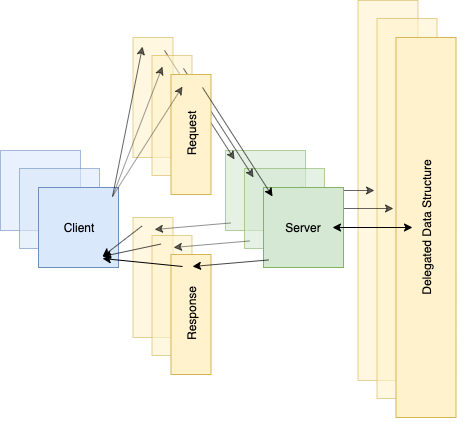
\includegraphics[width=0.9\columnwidth]{FIG/general_delegation.png}
\caption{A delegation system with 3 clients and 3 servers. The foreground client makes a request to all three servers. }
\label{fig:general_delegation}
\end{figure}
Delegation, as described in \cite{ffwd}, provides exclusive control over a data structure to a single thread called a \textit{server}. Servers receive requests to perform an operation on their memory from other threads called \textit{clients} via a 64 Byte struct containing a function pointer, up to 6 arguments, and a status flag. Similarly responses are communicated via a 16 Byte struct containing a return value and a status flag.  

Every server-client pair has at least one dedicated request line and one dedicated response line. ~\ref{fig:general_delegation} shows a system with 3 clients and 3 servers. The client in the foreground makes a request to its allocated request line on all three servers. The server performs an operation on its delegated data structure, and writes the response to the response line allocated to that specific client. Since each request and response line has only one writer, there is no data race nor any cache line contention. 

Each delegation \textit{server} iterates through an array of requests. When a new request is encountered the server loads the parameter values included in the request to the appropriate registers and then calls the function pointer. The server stores the return value from the function and the flag variable into an array of responses. 

Programs using the delegation library typically initialize the data structure to delegate, launch the dedicated servers, and then launch threads running the client function through a POSIX threads like interface. 

%\textit{Clients} maintain an array of request pointers targeting the client's assigned request line on each server. \textit{Clients} also maintain an array of pointers to the servers' responses. A client identifies a response is ready when it reads that the flag in the response is equal to the value it was set to in the request. 

An advantage of delegation is spatial locality of memory. A block of memory accessed exclusively by a delegation server is never shared with another thread. When the delegated memory block is sufficiently small, the entire working memory may fit within a server's higher levels of cache and remain resident for the duration of the program. In contrast, a system with multiple physical cores accessing the same size memory block will share cache lines, greatly reducing the likelihood of a higher level cache hit. 

From the client perspective, a drawback of delegation is the latency from request issuance to response. In ffwd, a synchronous delegation system, clients issue a request to the server's request line and then poll the respective response line until the request is returned. The time to complete a single delegated operation includes the time to write to the server, perform the function, and then receive the response. 

Gepard introduces concurrency in delegation operations while maintaining a synchronous appearance to the programmer by enabling a thread to switch to productive work through the use of fibers. Based upon \cite{libfiber}, fibers are light-weight, cooperatively scheduled user mode threads. Gepard clients write a delegation request to the server then make a rapid context switch to another working client fiber. After some time the client fiber will be reactivated, read its response, and then continue execution. The major advantage of \textit{Gepard} is that it enables a single thread to engage with multiple servers concurrently; increasing throughput despite constant individual request latency. 

In \textit{Gepard} and \textit{FFWD} the client application blocks after issuing a request until a response is received from the server. \textit{Gepard} hides the latency of the request by switching fibers during this waiting period. However if we can tolerate an asynchronous programming model we can expose greater concurrency without the overhead of switching user space fibers. 

%Gepard shows XXpc increased throughput from ffwd on XX benchmark by issuing parallel requests. However, we see that Gepard servers are capable of handling many more requests per second than can be provided by Gepard clients if the programmer can tolerate an asynchronous paradigm.  

\chapter{Asynchronous Delegation}
\subsection{General}
\begin{table}[ht!]
\begin{tabularx}{\linewidth}{| r | X |} %{ | p{2.5 in} p{4 in} | }
  \hline
  \bf{Function} & \bf{Description} \\
  \hline
  \bf{Launch\_Servers(n)} & Starts the specified number of server threads, allocates and initializes the request and response lines. \\
  \hline
  \bf{Delegate\_Thread\_Create(f, arg)} & Allocates and initializes a pending request queue for every server as thread local variable. Launches an OS thread to run function f with argument arg. \\
  \hline
  \bf{Delegate\_Async(s, cb, f, args...)} & Generates a delegation request to server s with function f and arguments args. Calls cb with the return value from f. \\
  \hline
  \bf{Delegate\_Async\_Barrier()} & Places requests from a delegated thread's queue and polls server responses until all requests have been served. \\
  \hline
\end{tabularx}
\label{tab:api}
\caption{Excerpt of the asynchronous delegation API}
\end{table}

The change offered by asynchronous delegation is evident in the difference in the API. While \textit{Gepard} and \textit{FFWD} make a call to \textbf{delegate(s, retval, f, args)} and block until a value is returned, asynchronous delegation makes a call to \textbf{Delegate\_Async(s, cb, f, args)} where cb is a callback function with the return value as a parameter. For most invocations a call to \textbf{Delegate\_Async(s, cb, f, args)} is non-blocking. 
An excerpt of the asynchronous delegation API is shown in ~\ref{tab:api}. 

In this chapter we will discuss the asynchronous delegation with one or more dedicated delegation server threads. Later, we will show how asynchronous operation can be applied to flat delegation, a more recent, serverless design. 

\section{Asynchronous Dedicated Delegation}
\begin{figure}[ht!]
\centering
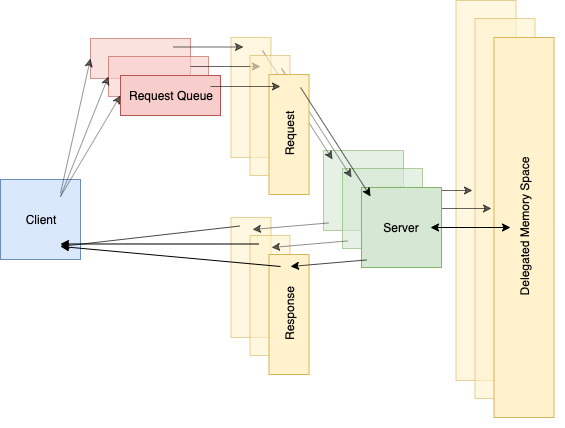
\includegraphics[width=0.9\columnwidth]{FIG/dedicated_async.png}
\caption{A delegation system with 1 client and 3 servers. The foreground client makes a request to all three servers. Requests are written to a pending request buffer which is periodically flushed out to the request line. }
\label{fig:dedicated_delegation}
\end{figure}

~\ref{fig:dedicated_delegation} demonstrates a dedicated delegation system with 1 client and 3 servers. In general, the client generates requests and places them in the fixed-length request queue for the required server. When any of the queues fills, the client will suspend request generation and begin the process of writing out requests to servers. The client polls its response lines one by one, executing the callback function if provided. Then a request is popped from the request queue and placed in the request line corresponding with the recently served response. After all response-request lines have been handled the client returns to generating requests. 

Specifically, to use dedicated delegation as shown in ~\ref{fig:dedicated_delegation}, the user must first initialize a number of delegation servers using \textbf{Launch\_Servers}. Running on separate OS threads, the servers begin sequentially polling their request lines. The user then launches OS threads with the application code by calling \textbf{Delegate\_Thread\_Create}. The thread launched by \textbf{Delegate\_Thread\_Create} first initializes an empty queue of pending requests for each running server on the NUMA node which the client thread is assigned. The queue is implemented as a fixed size circular buffer to take advantage of the prefetcher by keeping memory consecutive requests in consecutive address.  After queue initialization the thread invokes the client function. 

Within the client function the programmer uses \textbf{Delegate\_Async} to delegate the request. Typically delegate async will enqueue the request locally and then return to the client function. However, when any of the pending request queues is filled, the client works through its entire list of responses. When a response is ready, the client invokes the callback with the corresponding return value, and then writes a new request to the corresponding request line from the pending request queue. 

At any time the user can call \textbf{Delegate\_Async\_Barrier} to ensure that all outstanding requests are served before moving on.  \textbf{Delegate\_Async\_Barrier} is always called after the return of the client function and before joining the client thread. 

\subsection{Design Parameters for Asynchronous Dedicated Delegation}
\begin{figure}[ht!]
\centering
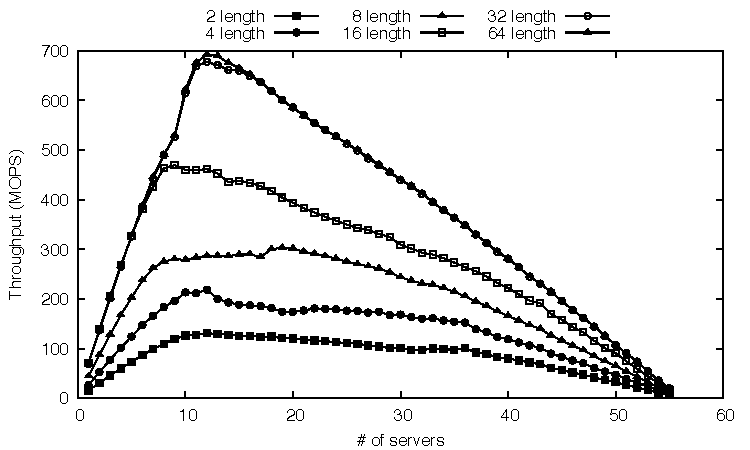
\includegraphics[width=0.9\columnwidth]{FIG/vary_queue_length.pdf}
\caption{Throughput in MOPS for a 56 thread system by number of servers by pending request queue length. The remainder of threads are clients.}
\label{fig:dedicated_vary_queue}
\end{figure}

\begin{figure}[ht!]
\centering
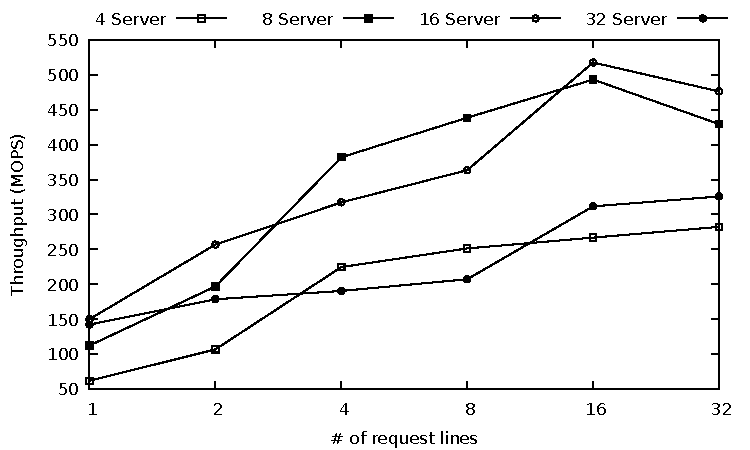
\includegraphics[width=0.9\columnwidth]{FIG/thput_by_rl.pdf}
\caption{Throughput in MOPS for a 56 thread system by number of request lines. }
\label{fig:dedicated_thput_by_rl}
\end{figure}

\begin{figure}[ht!]
\centering
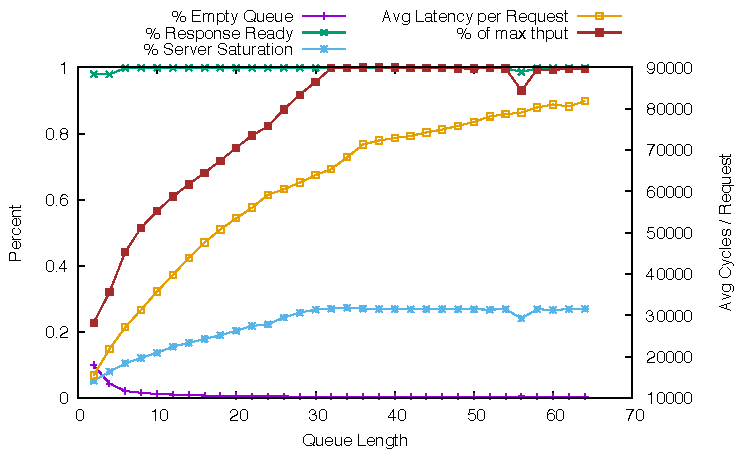
\includegraphics[width=0.9\columnwidth]{FIG/16rldedicated_saturation.pdf}
\caption{Latency, Server Saturation, Response Readiness, and Failed Queue Pops by queue length.}
\label{fig:saturation16RL}
\end{figure}

A feature of dedicated delegation is the ability to select the number of clients and servers operating in the system. This is a course grained way for the programmer to balance the expected request production rate of a client with the expected consumption rate of the server. Ideally the throughput of the system would follow the equation: 
\begin{displaymath}
Thput_{system} = \min(N_{server} * Thput_{server}, N_{client} * Thput_{client})
\end{displaymath}
Where Thput\textsubscript{system} is the throughput of the entire system in MOPS, Thput\textsubscript{component} is the throughput of an individual component in MOPS, and N\textsubscript{component} is the number of that component in the system.  

~\ref{fig:dedicated_vary_queue} shows the results of tests demonstrating this relationship. In this test, each server is delegated a 64 B variable. The clients operate for a fixed period of time, selecting a server at random and sending a request to increment the variable. In this test the sum of clients and servers in the system always sums to 56.

In the regions left of peak throughput shown in  ~\ref{fig:dedicated_vary_queue} the system is bound by server capacity. The upward slope corresponds to the consumption rate of an individual server, or Thput\textsubscript{server}. Conversely, in the region to the right of peak throughput the system is bound by client production. The downward slope corresponds to the Thput\textsubscript{client}. 

Beyond using more servers for concurrency, we can adjust the number of requests that can be sent to any one server at a given time by increasing the number of request lines. a server polls while in operation. ~\ref{fig:dedicated_thput_by_rl} shows the measured system throughput for the same benchmark described above by the number of request lines per server-client pair. ~\ref{fig:dedicated_thput_by_rl} shows that increasing the number of request line generally increases the throughput until about 16 request lines when performance degrades. Due to this observation we use 16 request lines for the rest of our experiments. 

From ~\ref{fig:dedicated_vary_queue} we see that increasing the length of the pending request queue clearly increases the throughput of the system. ~\ref{fig:saturation16RL} shows the saturation of the server, or rate of ready requests to request line reads for a system running the same benchmark with 16 servers and 40 clients. Server saturation increases with the extension of the pending request queue. The servers are simply doing more work with fewer reads. 

~\ref{fig:saturation16RL} also provide insight into the relationship between the pending request queue length and overall throughput shown in ~\ref{fig:dedicated_vary_queue}. \textbf{Delegate\_Async()} blocks to read responses and write requests whenever a push to any of its request queues fails. Ideally, \textbf{Delegate\_Async()} should block at a frequency slow enough that servers have had time to execute the outstanding responses and cache many requests to write concurrently but fast enough that responses do not age on the response line. 

The probability that \textbf{Delegate\_Async()} will block with slower frequency increases with the length of the request queue. The probability, P, that a system with S queues of length L will block after L total requests follows $ P = \frac{S}{L^{S}} $. Clearly the probability of stopping after L total requests drops rapidly as the queue length increases. Intuitively, this also provides the opportunity for requests to be cached across a range of servers. When the queue is sufficiently long and there is diversity in requests, we have a good probability that each queue will hold requests to fill all the request lines when \textbf{Delegate\_Async()} blocks. 

~\ref{fig:saturation16RL} confirms all of the above desirable traits of the queue length. As the queue length increases, the proportion of failed queue pop operations to successful one plummets. The increased period between response line polls also results in higher response availability. More requests are written to the server, with server occupancy topping out at 60\%. After increasing pending request queue length to double the number of request lines, however, the benefits of the longer queue begin to erode. This is shown by the 64 length queue in ~\ref{fig:dedicated_vary_queue}. When the queue is too long it acts like a reservoir, impounding requests for a longer period of time without impacting the throughput of the system. This is shown in ~\ref{fig:saturation1RL} and \ref{fig:saturation16RL} by the increase in individual request latency as the queue length increases. 

As a rule of thumb, we set the pending request queue to double the amount of request lines per client - server pair. This configuration provides high throughput while leaving cache available for delegated data structures. 

\subsection{Comparison with Gepard}
While \textit{Gepard} provides concurrency via a context switch during its blocking \textbf{Delegate} call, asynchronous delegation decouples the request and response polling altogether. The difference is that asynchronous delegation can enqueue a 64 B  request while \textit{Gepard} must preserve a 1 KB stack and spend processor time on the context switch. Besides the advantage of running significantly fewer instructions per operation, the much smaller memory footprint of asynchronous delegation increases the amount of cache available for delegated data structures when sharing a physical core with a delegation server.  % Validate these claims

\section{Asynchronous Flat Delegation}
\begin{figure}[ht!]
\centering
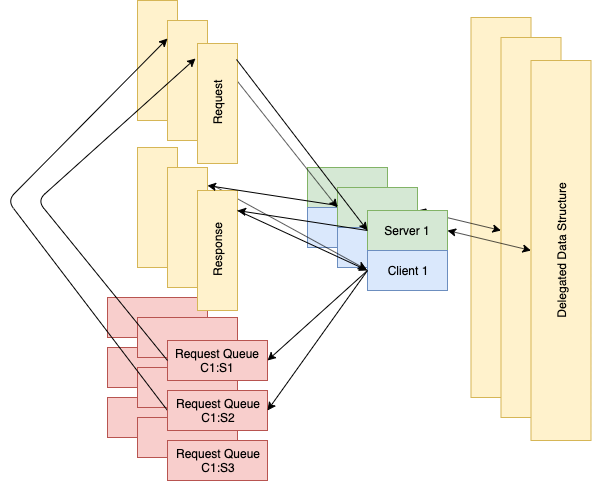
\includegraphics[width=0.9\columnwidth]{FIG/flat_async.png}
\caption{A flat delegation system with 3 client-server threads. The foreground client makes a request to itself. The background client makes a request to the foreground server. }
\label{fig:flat_delegation}
\end{figure}

Flat delegation combines the client and server roles of dedicated delegation into a single thread. The goal is to simplify delegation programming by finding a natural equilibrium between client and server rather than the user specified client to server ratio of dedicated delegation. ~\ref{fig:flat_delegation} sketches a sample flat delegation system with three OS threads splitting duty as client and server. Functions performing client and server duty are called from the same thread represented by the split box in the center of the figure. In ~\ref{fig:flat_delegation} the client generates requests and writes them out to the request line of the desired server, which may be the server to be invoked later on the same thread. Depending on the scheduling policy, the server function will be called to handle the requests on its request line. 

Since flat delegation does not launch dedicated server threads there is no call to \textbf{Launch\_Servers}. Besides this difference the API remains the same as dedicated delegation. 

\subsection{Design Parameters for Flat Delegation}  

\begin{figure}[ht!]
\centering
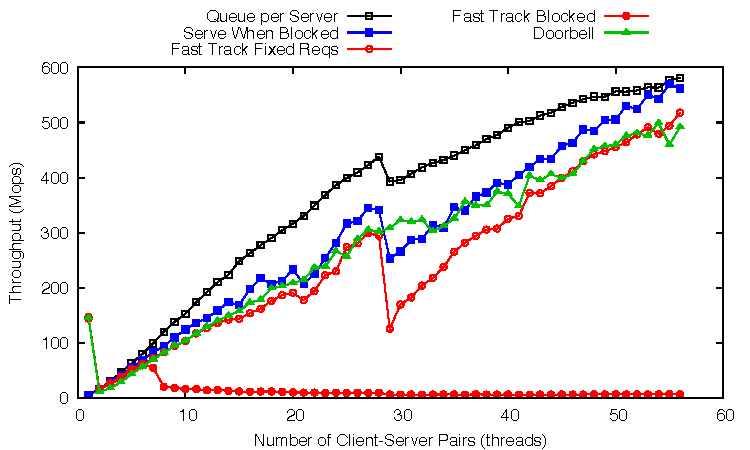
\includegraphics[width=0.9\columnwidth]{FIG/flat_delegation_strategy.pdf}
\caption{Flat delegation throughput by scheduling policy.}
\label{fig:flat_delegation_strategy}
\end{figure}

Although the API for asynchronous flat delegation remains the same, within \textbf{Delegate\_Async()} the client must write out requests and determine when to invoke the server function. Flat delegation servers run periodically as determined by the scheduling policy instead of continuously as they do in the dedicated approach. Because of this key difference, we experimented with writing requests to servers directly and also with different strategies for invoking the server function. 

The main difference we've made to writing requests is to issue them directly to the server's request line. To write the request the client keeps track of the most recently used request line on a server. Upon a \textbf{Delegate\_Async} call, the next response line is handled if available. After handling the response, if the request line is free the request is written out. An unavailable request line signifies that the remote server has not run for some time. 

Perhaps the simplest strategy for invoking the server function is upon a failed request issuance. After all, if the client is \textit{blocked} waiting for a server to become available, the most useful thing it can do is run the server itself. 

A proposed optimization to the serve when blocked policy was to fast track requests to a server on the same thread as the client by invoking the delegated function directly. The unintended impact of this optimization was the \textit{greedy} client problem, which is caused by victim threads attempting to write requests to the full request lines of the greedy client. The victim threads operate in server mode until the request line becomes available. However, the request line never becomes available because the greedy client's requests continue to be served by the victim threads. The greedy client problem was avoided in the serve when blocked strategy because the client was guaranteed to invoke the server function when writes to the request lines of its own server blocked. The fast track eliminated this natural trigger. 

To break the greedy client we experiment with an upper \textit{bound} on the client by invoking the server after a fixed number of calls to \textbf{Delegate\_Async()}. We also implement the \textit{doorbell} strategy. When a client blocks on an unavailable request line it "rings the doorbell" of the required thread by writing a 1 to its doorbell variable. Clients check their doorbell during each call to \textbf{Delegate\_Async} and invoke the server, resetting the doorbell to zero after a run of the server loop.

We test each of these strategies using the same benchmark described in \ref{Design Parameter for Asynchronous Dedicated Delegation}. The results of the trials with five different scheduling strategies are summarized in ~\ref{fig:flat_delegation_trials}. Note that the horizontal axis describes the number of client server pairs, which is also the total number of threads running in the system. The \textit{queue} strategy exhibits the highest throughput throughout the range of threads used on the system, although the serve when \textit{blocked} strategy showed comparable performance for larger numbers of threads. 

The \textit{blocked} strategy exhibits a desirable property shown in ~\ref{fig:flat_latency_56} and ~\ref{fig:flat_latency_28}: The latency for any individual request, from generation to execution of the callback function is 16.8\% lower for \textit{blocked} than \textit{queue}. 

\begin{figure}[ht!]
\centering
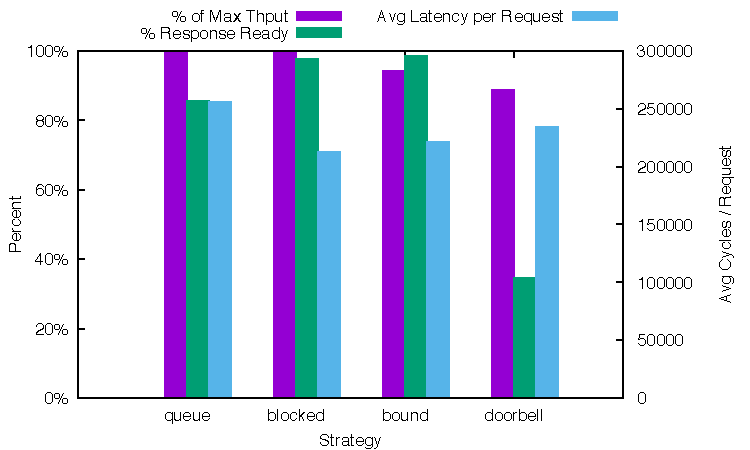
\includegraphics[width=0.9\columnwidth]{FIG/flat_latency_56.pdf}
\caption{56 server-client pair comparison of average request latency, response line availability, and comparative throughput. Greedy omitted for scale.}
\label{fig:flat_latency_56}
\end{figure}

\begin{figure}[ht!]
\centering
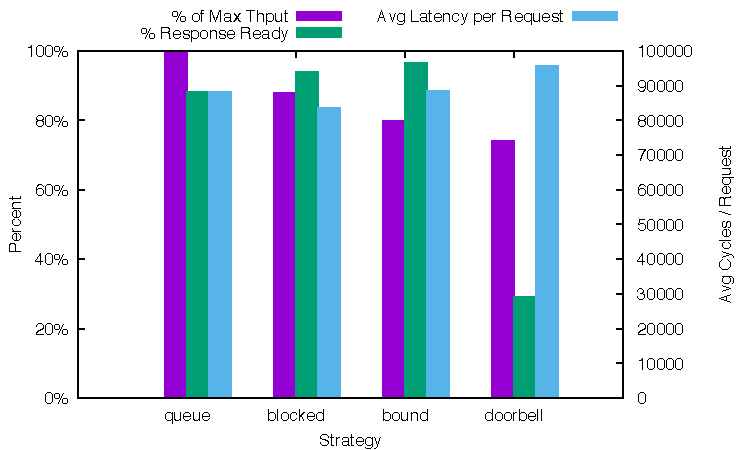
\includegraphics[width=0.9\columnwidth]{FIG/flat_latency_28.pdf}
\caption{28 server-client pair comparison of average request latency, response line availability, and comparative throughput. Greedy omitted for scale.}
\label{fig:flat_latency_28}
\end{figure}

\section{Ordering Guarantees}
\begin{figure}[ht!]
\centering
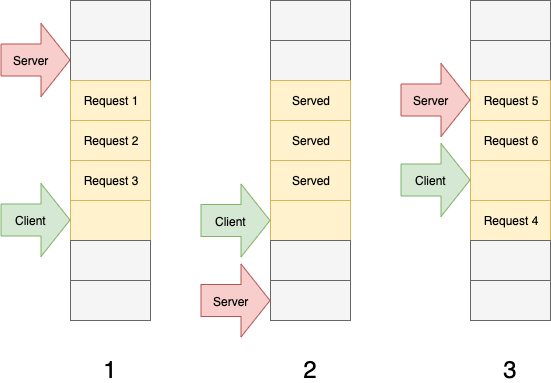
\includegraphics[width=0.9\columnwidth]{FIG/multiple_rl_race.png}
\caption{The server may execute requests out of order when multiple requests lines are used by one client. (1.) The client issues 3 requests before the server reaches its section of the request line array. (2.) The server handles all requests in this clients section before the client writes a fourth request. (3.) The client writes its next request into the next available line, after request 4 is written the next line is the first one. The requests are now executed out of order.}
\label{fig:mulitple_rl_race}
\end{figure}
The asynchronous API provides no guarantee to the ordering of delegated functions. Delegated functions may be executed out of generation order when delegated to different servers because the servers are not synchronized with respect to each other. Even requests to the same server may be reordered as described below.  

Servers handle requests by iterating through all of their request lines and performing those requests with the appropriate flag. However, when there are multiple request lines per server-client pair we cannot guarantee that the requests will be performed in the order they are sent. Consider the case shown in ~\ref{fig:multiple_rl_race}.  A client writes a request to all but one of its request lines before the server handles the entire batch. Afterward the client writes requests to its last request line and then begins writing new requests to its first request line. Since the server handles requests in the order of the request line array, newer requests are handled before the oldest request in the last position. 

For an application with non-commutative properties, the programmer can take care to delegate the entire order critical section. It that is unfeasible, a single request line preserves the ordering of requests made by a client to a specific server. Experimental results are shown with both 1 and 16 request lines per client-server pair to show the difference in throughput while maintaining ordering. 

\chapter{Experimental Evaluation}
The following results shown are from a 28 core, 56 thread Intel Skylake machine with 97 GB of RAM, 32kB of L1 cache, 1,024KB of L2 cache, and 19,712kB L3 cache shared among the 14 physical cores on each socket. 

For locking, atomic operations, and flat delegation we use the number of threads available on the machine (56) unless stated otherwise. For trials with the dedicated organization we list the number of servers. The balance of remaining threads are clients.  The client and server ratio is selected by the best results with 1 variable per server. 

Like \textit{Gepard}, asynchronous delegation threads are assigned to cores in a round-robin fashion. In the dedicated case all server threads are launched before any client threads. Memory for delegated data structures is allocated on the NUMA node corresponding to the server which it is assigned. 

Results shown are the weighted arithmetic mean performance over 10 runs of three seconds or greater. 

\section{Fetch and Add Performance}
\begin{figure}[ht!]
\centering
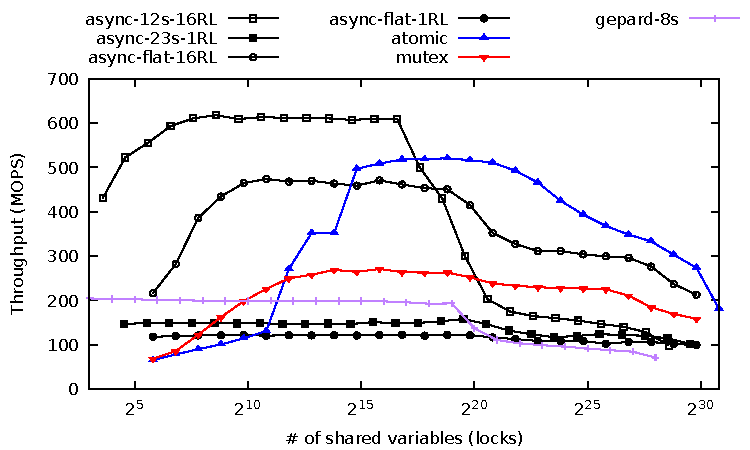
\includegraphics[width=0.9\columnwidth]{FIG/fetch_and_add_thput.pdf}
\caption{Throughput in MOPS by number of 64Byte variables. Higher is better. }
\label{fig:fetch_and_add_thput}
\end{figure}

The experiment shown in ~\ref{fig:fetch_and_add_thput} selects a variable at random and then increments it using the synchronization type shown. Each variable is 64 Bytes and 64 Byte aligned. The locking cases are the posix mutex and spin lock. For the locking case the lock takes the place of padding in the variable struct. There is one lock per variable. In cases where variables cannot be delegated evenly, the number of variables is rounded up to the nearest multiple of the number of servers. 

Delegation approaches excel for smaller numbers of shared variables. Notice dedicated delegation achieves over 600 MOPS for shared variable counts up to the size of the server cache. Flat delegation achieves consistent performance, topping out near 500 MOPS. The reason for this even performance at low levels of shared variables is a lack of contention.

\begin{figure}[ht!]
\centering
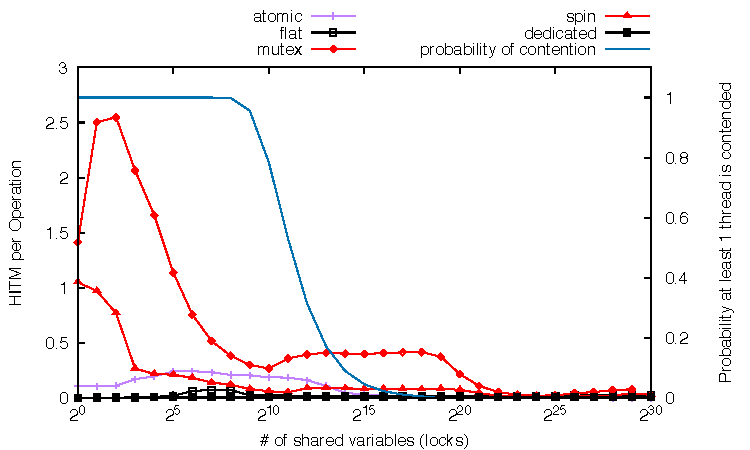
\includegraphics[width=0.9\columnwidth]{FIG/hitm_per_op.pdf}
\caption{Remote hitm L3 cache invalidations by variable size. }
\label{fig:contention}
\end{figure}

A variable is contended if multiple threads are trying to access it simultaneously. Neglecting interleaving due to time, the chance that at least one pair of threads in the system are contending for a variable is plotted in ~\ref{fig:contention} and described as follows. : 
\begin{displaymath}
contention = 1 - {{ variables \choose threads }  \over  variables^{threads}}
\end{displaymath}


The fine grained locks and the atomic fetch and add have up to 56 threads accessing a single memory location. ~\ref{fig:fetch_and_add_thput} shows the atomic fetch and add and the fine grained locks reach peak performance as the probability of contention reaches 0 ~\ref{fig:contention}. In our microbenchmark, where each thread executes transactions at random, we can assume contention for variables among cores renders the L1 and L2 cache useless because the cache lines are constantly being invalidated by competing cores. We can observe this behavior in the number of L3 lines invalidated by a remote processors L3 cache. 

In contrast, the delegation approaches, by design, have no contention for variables. When the number of shared variables is sufficiently small, the entire data set may be kept in a core's L1 and L2 cache. For the 16 server dedicated delegation case shown, each delegation server shares, as a hyperthread, a core with a delegation client. The combined overhead of the two threads is about 93 kB. This amount consumes the entire L1 cache and 62 kB of the L2. This leaves 962 kB of L2 cache for data. 960 kB translates to 15 k variables per server, or 246 k variables for the system. L2 cache should be exhausted at 2\textsuperscript{18} variables, which is where we see the performance begin to degrade. Further, the portion of L3 cache available to the server is roughly 1 / N\textsubscript{server on processor} of the L3 on the processor, or 2,464 kB. This translates to 39 k additional variables per server, or 630 k more variables for the system. L3 is exhausted when the number of shared variables approaches 2\textsuperscript{20}. Performance continues to degrade as the number of variables resident in DRAM increases and the likelihood of cache hits decreases. 

%For quantities of shared variables smaller than the size of a single processors cache contention should be evident in L3 cache hits. More L3 cache hits indicate more contention because uncontended variables should remain in a processors exclusive L1 or L2 cache. ~\ref{fig:contention} shows delegation approaches with fewer L3 cache hits per operation compared to the atomic fetch and add and the fine grained mutex lock. 

\begin{figure}[ht!]
\centering
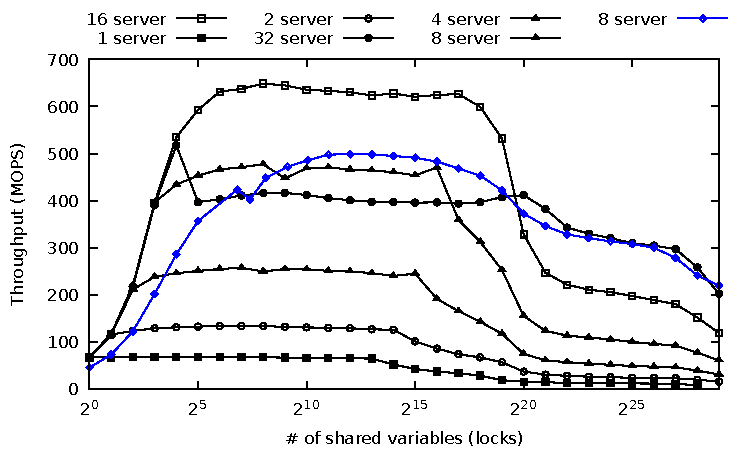
\includegraphics[width=0.9\columnwidth]{FIG/fetch_add_dedicated_vary_server.pdf}
\caption{Throughput by Shared Variables by Number of Dedicated Servers}
\label{fig:vary_server}
\end{figure}

A variable is contended if multiple threads are trying to access it simultaneously. Neglecting interleaving due to time, the chance that at least one pair of threads in the system are contending for a variable is plotted in ~\ref{fig:contention} and described as follows. : 
\begin{displaymath}
contention = 1 - {{ variables \choose threads }  \over  variables^{threads}}
\end{displaymath}

A common theme across all approaches is the degradation of performance beginning around 2\textsuperscript{20} shared variables. Due to the randomness in the benchmark, the probability that an approach will be reading from DRAM nears 1 as the number of shared variables increases. Much slower access to DRAM dominates the performance of all approaches in this region, however the degradation in performance is particularly extreme for dedicated delegation because accesses are made by a smaller subset of cores. ~\ref{fig:vary_server} shows as the number of server cores increases the tail performance of dedicated delegation improves. 

%The microbenchmark accesses variables at random, so we will assume as the number of shared variables exceeds the amount of cache in the system that it is likely a variable will be evicted from cache before it is accessed again. 

In a similar vein, a strength of flat delegation is its ability to utilize every core in the machine for DRAM access. Flat delegation also benefits from the lower cycle time for an on NUMA Node DRAM access. In comparison, the spin lock or compare and swap will have a 1:N\textsubscript{NUMA Nodes} probability of picking a variable at random that is addressed on the same node as the core. A FIGURE I HAVENT MADE YET shows the number of accesses to remote dram per operation by approach. 

\begin{displaymath}
{P_{In Cache}} = {{L2BytesAvailable} \over { size of shared variables / number of servers}}
\end{displaymath}
As the probability that a variable is in cache approaches zero the time to access DRAM dominates the performance of the delegation server. Flat delegation offers an improvement to other delegation designs in this region because it maintains the same number of threads making memory accesses while ensuring that all DRAM access are local to the thread's NUMA node. 

% Figure - DRAM Accesses by program by variable count
% Run and discuss the Hash Map here. 
Where atomic operations are unfeasible, we would expect flat delegation to outperform all other options for the extreme end of the range. 





The 16 request line case in ~\ref{dedicated_thput_client_server} exhibits the expected behavior. ~\ref{fig:dedicated_thput_client_server} shows the throughput for a simple fetch and add benchmark by increasing number of servers. In the region of the positive slope the system bottleneck is the server capacity. Each additional server added increases the system throughput by the individual server consumption rate. Conversely the region of the negative slope indicates the system bottleneck to be client production capacity. After peak throughput is achieved, reassignment of a client to server duty reduces the system throughput by the individual client production rate. The throughput peaks when the combined server consumption rate matches the combined production rate of the clients. 

The dedicated design stores requests in an array of local queues, one for each server in the system (see ~\ref{fig:dedicated_delegation}).  When one of the queues is full, the client writes as many requests as it can.  FIGURE shows the effect of the queue length on the fetch and add microbenchmark. As the queue length increases, the system achieves greater throughput. This is because the probability of all queues having any requests present increases as the queue length increases. When servers are picked at random, the probability of stopping to flush the queues when only one queue contains requests is as follows: 
\begin{displaymath}
P(Full Queue) = {N_{queues} \over {N_{queues}}^{L_{queue}}}
\end{displaymath}

%This is because the longer queue lengths allow more requests to accumulate in each server queue before the requests are written out to the servers. Writing more requests at once brings greater efficienct to the client, as evidenced by the shallower slope of the ... 

%Production Rate - Client
%Consumption Rate - Server

Figure: max throughput by client-server combination for all cores case
	Discussion production rate of clients, consumption rate of clients
Figure: Throughput by number of request lines
Figure: Throughput by size of ring buffer, no ring buffer
	Server and Client hit rate

\section{Design Parameters for Flat Delegation}

Instead of specifying the 

Figure: Throughput by schedule type
	Server and client hit rate

\chapter{Conclusions}
Flat provides and easier API, no tuning. 
%Validate - does it extend the performance for larger data structures?
Dedicated allows the user to adjust the producer / consumer rates
Applications are programs with smallish data structures with operations more complicated than compare and swap. 


%\chapter{Some other stuff I wrote but probably shouldn't be included}
%\section{Hardware}
%Under consideration is our highly parallel machine consisting of multiple processing units, or cores, sharing resources on a single silicon processor. Cores execute threads, or sequences of machine instructions. X86 machines often support the simultaneous execution of two threads at the same time. In this hyperthreaded scenario a core's resources are shared between the threads in execution. 
%
%Processors are installed in sockets on the machine's motherboard. The processors on separate sockets communicate with each other through a bus. On a machine supporting Non Uniform Memory Access (NUMA) each socket is also a NUMA Node, with direct access to a portion of main memory (DRAM). Cores on a socket will experience greater latency accessing memory addresses on a remote NUMA node than memory addresses resident on their local NUMA node because of the time required for the data to travel across the bus. 
%
%Access to main memory is a bottleneck for modern processors, which can perform an operation in as little as 1 cycle but write to memory in the order of LOOK THIS UP. To close this latency gap processors and cores have levels of cache, small amounts of high speed memory located closer to the processing unit. Cache is typically allocated in three levels, with levels 1 and 2 dedicated to a single core, while level 3 is shared among all cores on a processor. The latency of access to levels 1, 2, and 3 is around 5, 15, 60 cycles respectively. 
%
%The cache optimization works by making a working copy of the data at a memory address and moving it into the lower latency memory closer to the core. The core can manipulate this memory locally and write it out to main memory when it is complete. When access to a memory address is predictable or frequent, data at memory addresses can be moved ahead of time, or prefetched, to the cache, and the core can benefit from the lower latency of the cache memory.   
%
%Although memory is byte addressed, the cache system manages information in 64 byte segments called cache lines. Caches are typically n-way set associative. A set can hold up to n cache lines which share a common portion of their memory address. 
%
%For example, a 32kB 8-way set associative cache has 512 cache lines split into 64 sets. Each set accepts memory addresses with bits 6-11 of the memory address in common. 
%
%When a cache is full, the least recently used cache line is evicted to a lower level cache or main memory in favor of a newer cache line. 
%
%When multiple cores access memory in the same cache line the copies resident in each core's cache may become inconsistent. Cores can snoop on another core's cache line status. If a core detects that a cache line has been modified on another core, the snooping core signals the modifying core which then forwards the modified cache line, causing an increase in access time\cite{IntelDevelopersManual}. In a concurrent program multiple cores may be writing to separate addresses resident in the same cache line. The cache line is shared between cores although the memory addresses are not. This false sharing of the memory addresses increases access latency for all cores operating on the cache line. 
%
%\section{Schemes for Shared Memory Access}
%Of course concurrent programs not only false share cache lines, they perform operations on the same memory addresses as well. Without careful synchronization by the programmer multiple cores can read and modify a memory address concurrently producing a non-deterministic result. Some of the methods for preventing this data race are described below. 
%% Locking
%Mutual Exclusion (Mutex) locks synchronize memory access through a variable that a thread must claim before moving forward with its data altering, or critical, section. When a competing thread views the lock as occupied it will wait to execute its critical section until it gets exclusive control of the lock. 
%
%There are several ways of implementing the MUTEX lock. // expand upon this.  
%
%Regardless of the implementation, synchronization schemes using locks suffer bottlenecks due to sharing the lock variable across multiple processors or sockets. In fine grained locking schemes these lock variables may take up a significant portion of memory (validate this). Additionally, memory modified in the critical section may reside in another cache, local DRAM, or another NUMA node's DRAM. 
%% Atomic Operations
%Atomic operations are those operations where 
%% Transactional Memory
%
%
%
%\chapter{Rates and System Performance}
%% Quantifying the client - server relationship
%% 



%This is how we cite a paper \cite{Farine20162243}.
%
%Below is the example of algorithm block.
%
%
%\IncMargin{1em}
%\begin{alprocedure}[!htp]
%\caption{FindFactionsAndInitiators}
%\SetKwInOut{Input}{input}\SetKwInOut{Output}{output}
%\Input{An adjacency matrix $E^*$ of dynamic network}
%\Output{ A time series of faction sets $\mathcal{F}^*$, and a time series of initiator sets $\mathcal{L}^*$ }
%\BlankLine
%\For{$i\leftarrow 1$ \KwTo $t^*$}{
%\textcolor{cyan}{\tcc*[h]{Get a matrix at time $t=i$} }
%
%$E \leftarrow E^*_{ t = i}$ \; 
%\textcolor{cyan}{\tcc*[h]{FindInitiators($E $) returns all nodes which have zero outgoing degree}}
%
%$\mathcal{L} \leftarrow$FindInitiators($E $) \;
%$\mathcal{F} = \emptyset$ \;
%\For{$l \in \mathcal{L}$}{
%\textcolor{cyan}{\tcc*[h]{FindReachNodeFrom($E,l$) returns all nodes which have any directed path to $l$}}
%
%$F_l\leftarrow$FindReachNodeFrom($E,l$) \;
%$\mathcal{F} = \mathcal{F} \cup \{F_l\}$
%}
%$\mathcal{F}^*_{t=i} = \mathcal{F}  $ and $\mathcal{L}^*_{t=i} = \mathcal{L}  $
%}
%\label{algo:FindFactionsAndInitiators}
%\end{alprocedure}\DecMargin{1em}
%
%
%The example of table is below.
%
%\begin{table}[!htp]
%\tiny
%\centering
%\caption{Table Caption1}
%\label{table:htestdes}
%\begin{tabular}{l|l|l|}
%\cline{2-3}
%                                                                                                                     & \cellcolor[HTML]{EFEFEF}\textbf{Method}                                    & \cellcolor[HTML]{EFEFEF}\textbf{Null hypothesis $H_0$}                                                                                          \\ \hline
%\multicolumn{1}{|l|}{}                                                                                               & $t$-test                                                                      & \begin{tabular}[c]{@{}l@{}}A sample has a normal distribution \\ with zero mean and unknown variance.\end{tabular}                              \\ \cline{2-3} 
%\multicolumn{1}{|l|}{}                                                                                               & \cellcolor[HTML]{EFEFEF}Sign test                                          & \cellcolor[HTML]{EFEFEF}A sample has a distribution with zero median.                                                                           \\ \cline{2-3} 
%\multicolumn{1}{|l|}{\multirow{-3}{*}{\textbf{\begin{tabular}[c]{@{}l@{}}Zero \\ mean/median \\ test\end{tabular}}}} & Wilcoxon signed rank test                                                  & A sample has a symmetric distribution around zero median.                                                                                       \\ \hline
%\multicolumn{1}{|l|}{}                                                                                               & \cellcolor[HTML]{EFEFEF}Kolmogorov-Smirnov test (KS test)                           & \cellcolor[HTML]{EFEFEF}A sample comes from a normal distribution.                                                                              \\ \cline{2-3} 
%\multicolumn{1}{|l|}{}                                                                                               & \begin{tabular}[c]{@{}l@{}}Chi-square \\ goodness-of-fit test\end{tabular} & \begin{tabular}[c]{@{}l@{}}A sample comes from a normal distribution \\ with a mean and variance estimated from a sample itself.\end{tabular}   \\ \cline{2-3} 
%\multicolumn{1}{|l|}{}                                                                                               & \cellcolor[HTML]{EFEFEF}Jarque-Bera test                                   & \cellcolor[HTML]{EFEFEF}\begin{tabular}[c]{@{}l@{}}A sample comes from a normal distribution \\ with an unknown mean and variance.\end{tabular} \\ \cline{2-3} 
%\multicolumn{1}{|l|}{\multirow{-4}{*}{\textbf{\begin{tabular}[c]{@{}l@{}}Normality \\ test\end{tabular}}}}           & Anderson-Darling test                                                      & A sample comes from a normal distribution.                                                                                                      \\ \hline
%\end{tabular}
%\end{table}
%
%
%
%\section{Support of leading faction}
%
%\begin{figure}[ht!]
%\centering
%\includegraphics[width=0.9\columnwidth]{FIG/CoorEventSup}
%\caption{An example of image in thesis }
%\label{fig:CoorEventSup}
%\end{figure}
%
%
% \appendices
% \newpage
% \appendix
%
% \chapter{Some Ancillary Stuff}
%
% Ancillary material should be put in appendices.
%
% \chapter{Some More Ancillary Stuff}
%
% Here is yet another appendix! Wahoo!

%\nocite{*}
\bibformb
\bibliography{BibFile}
\newpage
% \vita
% This is where the vita goes.  Its organization is left as an exercise.
\clearpage
    \pagestyle{pageontop}
   \thispagestyle{pageonbottom}
   %\vspace*{3in}
   \begin{large}
   \begin{center}
   {\bfseries VITA}
   \end{center}
   \end{large}
\begin{tabular}{p{2.8cm}p{10.5cm}}
NAME: & NAME LASTNAME  \\ 
    &\\
EDUCATION:  &Ph.D., Computer Science, University of Illinois at Chicago, Chicago, Illinois, 2018. \\  
            &\\
            &M.Eng., Computer Engineering, University of Illinois at Chicago, Chicago, Illinois, 20xx.\\
            &\\
            &B.Eng., Computer Engineering, University of Illinois at Chicago, Chicago, Illinois, 20xx.  \\
            &\\
ACADEMIC EXPERIENCE:  &Research Assistant, Computational Population Biology Lab, Department of Computer Science, University of Illinois at Chicago, xxxx - 2018. \\
            &\\
            &Teaching Assistant, Department of Computer Science, University of Illinois at Chicago: \\
            &\squishlist            
            \item Computer Algorithm I, Spring xxxx and  Fall xxxx.    
            \item Secure Computer Systems, Fall xxxx 
            \squishend \\
            

 \end{tabular}

\end{document}
